% Options for packages loaded elsewhere
\PassOptionsToPackage{unicode}{hyperref}
\PassOptionsToPackage{hyphens}{url}
%
\documentclass[
  12pt,
]{article}
\usepackage{amsmath,amssymb}
\usepackage{lmodern}
\usepackage{ifxetex,ifluatex}
\ifnum 0\ifxetex 1\fi\ifluatex 1\fi=0 % if pdftex
  \usepackage[T1]{fontenc}
  \usepackage[utf8]{inputenc}
  \usepackage{textcomp} % provide euro and other symbols
\else % if luatex or xetex
  \usepackage{unicode-math}
  \defaultfontfeatures{Scale=MatchLowercase}
  \defaultfontfeatures[\rmfamily]{Ligatures=TeX,Scale=1}
\fi
% Use upquote if available, for straight quotes in verbatim environments
\IfFileExists{upquote.sty}{\usepackage{upquote}}{}
\IfFileExists{microtype.sty}{% use microtype if available
  \usepackage[]{microtype}
  \UseMicrotypeSet[protrusion]{basicmath} % disable protrusion for tt fonts
}{}
\makeatletter
\@ifundefined{KOMAClassName}{% if non-KOMA class
  \IfFileExists{parskip.sty}{%
    \usepackage{parskip}
  }{% else
    \setlength{\parindent}{0pt}
    \setlength{\parskip}{6pt plus 2pt minus 1pt}}
}{% if KOMA class
  \KOMAoptions{parskip=half}}
\makeatother
\usepackage{xcolor}
\IfFileExists{xurl.sty}{\usepackage{xurl}}{} % add URL line breaks if available
\IfFileExists{bookmark.sty}{\usepackage{bookmark}}{\usepackage{hyperref}}
\hypersetup{
  pdftitle={L3 French vowel categorization of L1 English-L2 Spanish speakers at absolute first exposure},
  hidelinks,
  pdfcreator={LaTeX via pandoc}}
\urlstyle{same} % disable monospaced font for URLs
\usepackage[margin=1in]{geometry}
\usepackage{graphicx}
\makeatletter
\def\maxwidth{\ifdim\Gin@nat@width>\linewidth\linewidth\else\Gin@nat@width\fi}
\def\maxheight{\ifdim\Gin@nat@height>\textheight\textheight\else\Gin@nat@height\fi}
\makeatother
% Scale images if necessary, so that they will not overflow the page
% margins by default, and it is still possible to overwrite the defaults
% using explicit options in \includegraphics[width, height, ...]{}
\setkeys{Gin}{width=\maxwidth,height=\maxheight,keepaspectratio}
% Set default figure placement to htbp
\makeatletter
\def\fps@figure{htbp}
\makeatother
\setlength{\emergencystretch}{3em} % prevent overfull lines
\providecommand{\tightlist}{%
  \setlength{\itemsep}{0pt}\setlength{\parskip}{0pt}}
\setcounter{secnumdepth}{-\maxdimen} % remove section numbering
\usepackage{tipa}
\usepackage{xcolor}
\ifluatex
  \usepackage{selnolig}  % disable illegal ligatures
\fi

\title{L3 French vowel categorization of L1 English-L2 Spanish speakers
at absolute first exposure}
\author{}
\date{\vspace{-2.5em}10/26/21}

\begin{document}
\maketitle

The present study investigates bilinguals' categorization of L3 sounds
at first exposure in order to inform debates in L3 phonological
acquisition. Models of third language acquisition debate the role of
previously known languages in the acquisition of a third. In particular,
the starting point of third language acquisition has been debated, in
which some models suggest that one language holistically influences the
L3 (The Typological Primacy Model; Rothman, 2015, the L2 Status Factor,
Bardel \& Falk, 2007), while others suggest that property-by-property or
gradient influence is possible (The Linguistic Priximity Model;
Westergaard et al., 2017, the Scalpel Model, 2017).

In the present study, participants who speak L1 American English and L2
Spanish completed a French vowel categorization task (Best \& Tyler,
2007, among others). Importantly, these participants did not speak
French, as the principle aim of the study was to assess the
cross-linguistic influence on perception at the initial state of L3
acquisition. During the task, they heard a total of 20 French vowel
sounds in 4 conditions (L1 bias, L2 bias, new sound, both languages) and
chose the closest matching L1 or L2 vowel sound given orthographically
in language-specific carrier words. Following a vowel selection, each
choice was rated for goodness of fit on a continuous scale.

The results revealed that novel L3 sounds are categorized using both L1
and L2 categories (Figure 1). Additionally, the same L3 sounds were not
always categorized the identically within subjects, nor were all
selections typically in one language (Figure 2). These results suggest
that both languages of a bilingual are active during L3 perceptual
routines and best support the Linguistic Proximity Model (Westergaard et
al., 2017), while providing counter-evidence for full transfer models of
L3 acquisition such as the L2 Status Factor and the Typological Primacy
Model.

\newpage

\textbf{Figure 1}

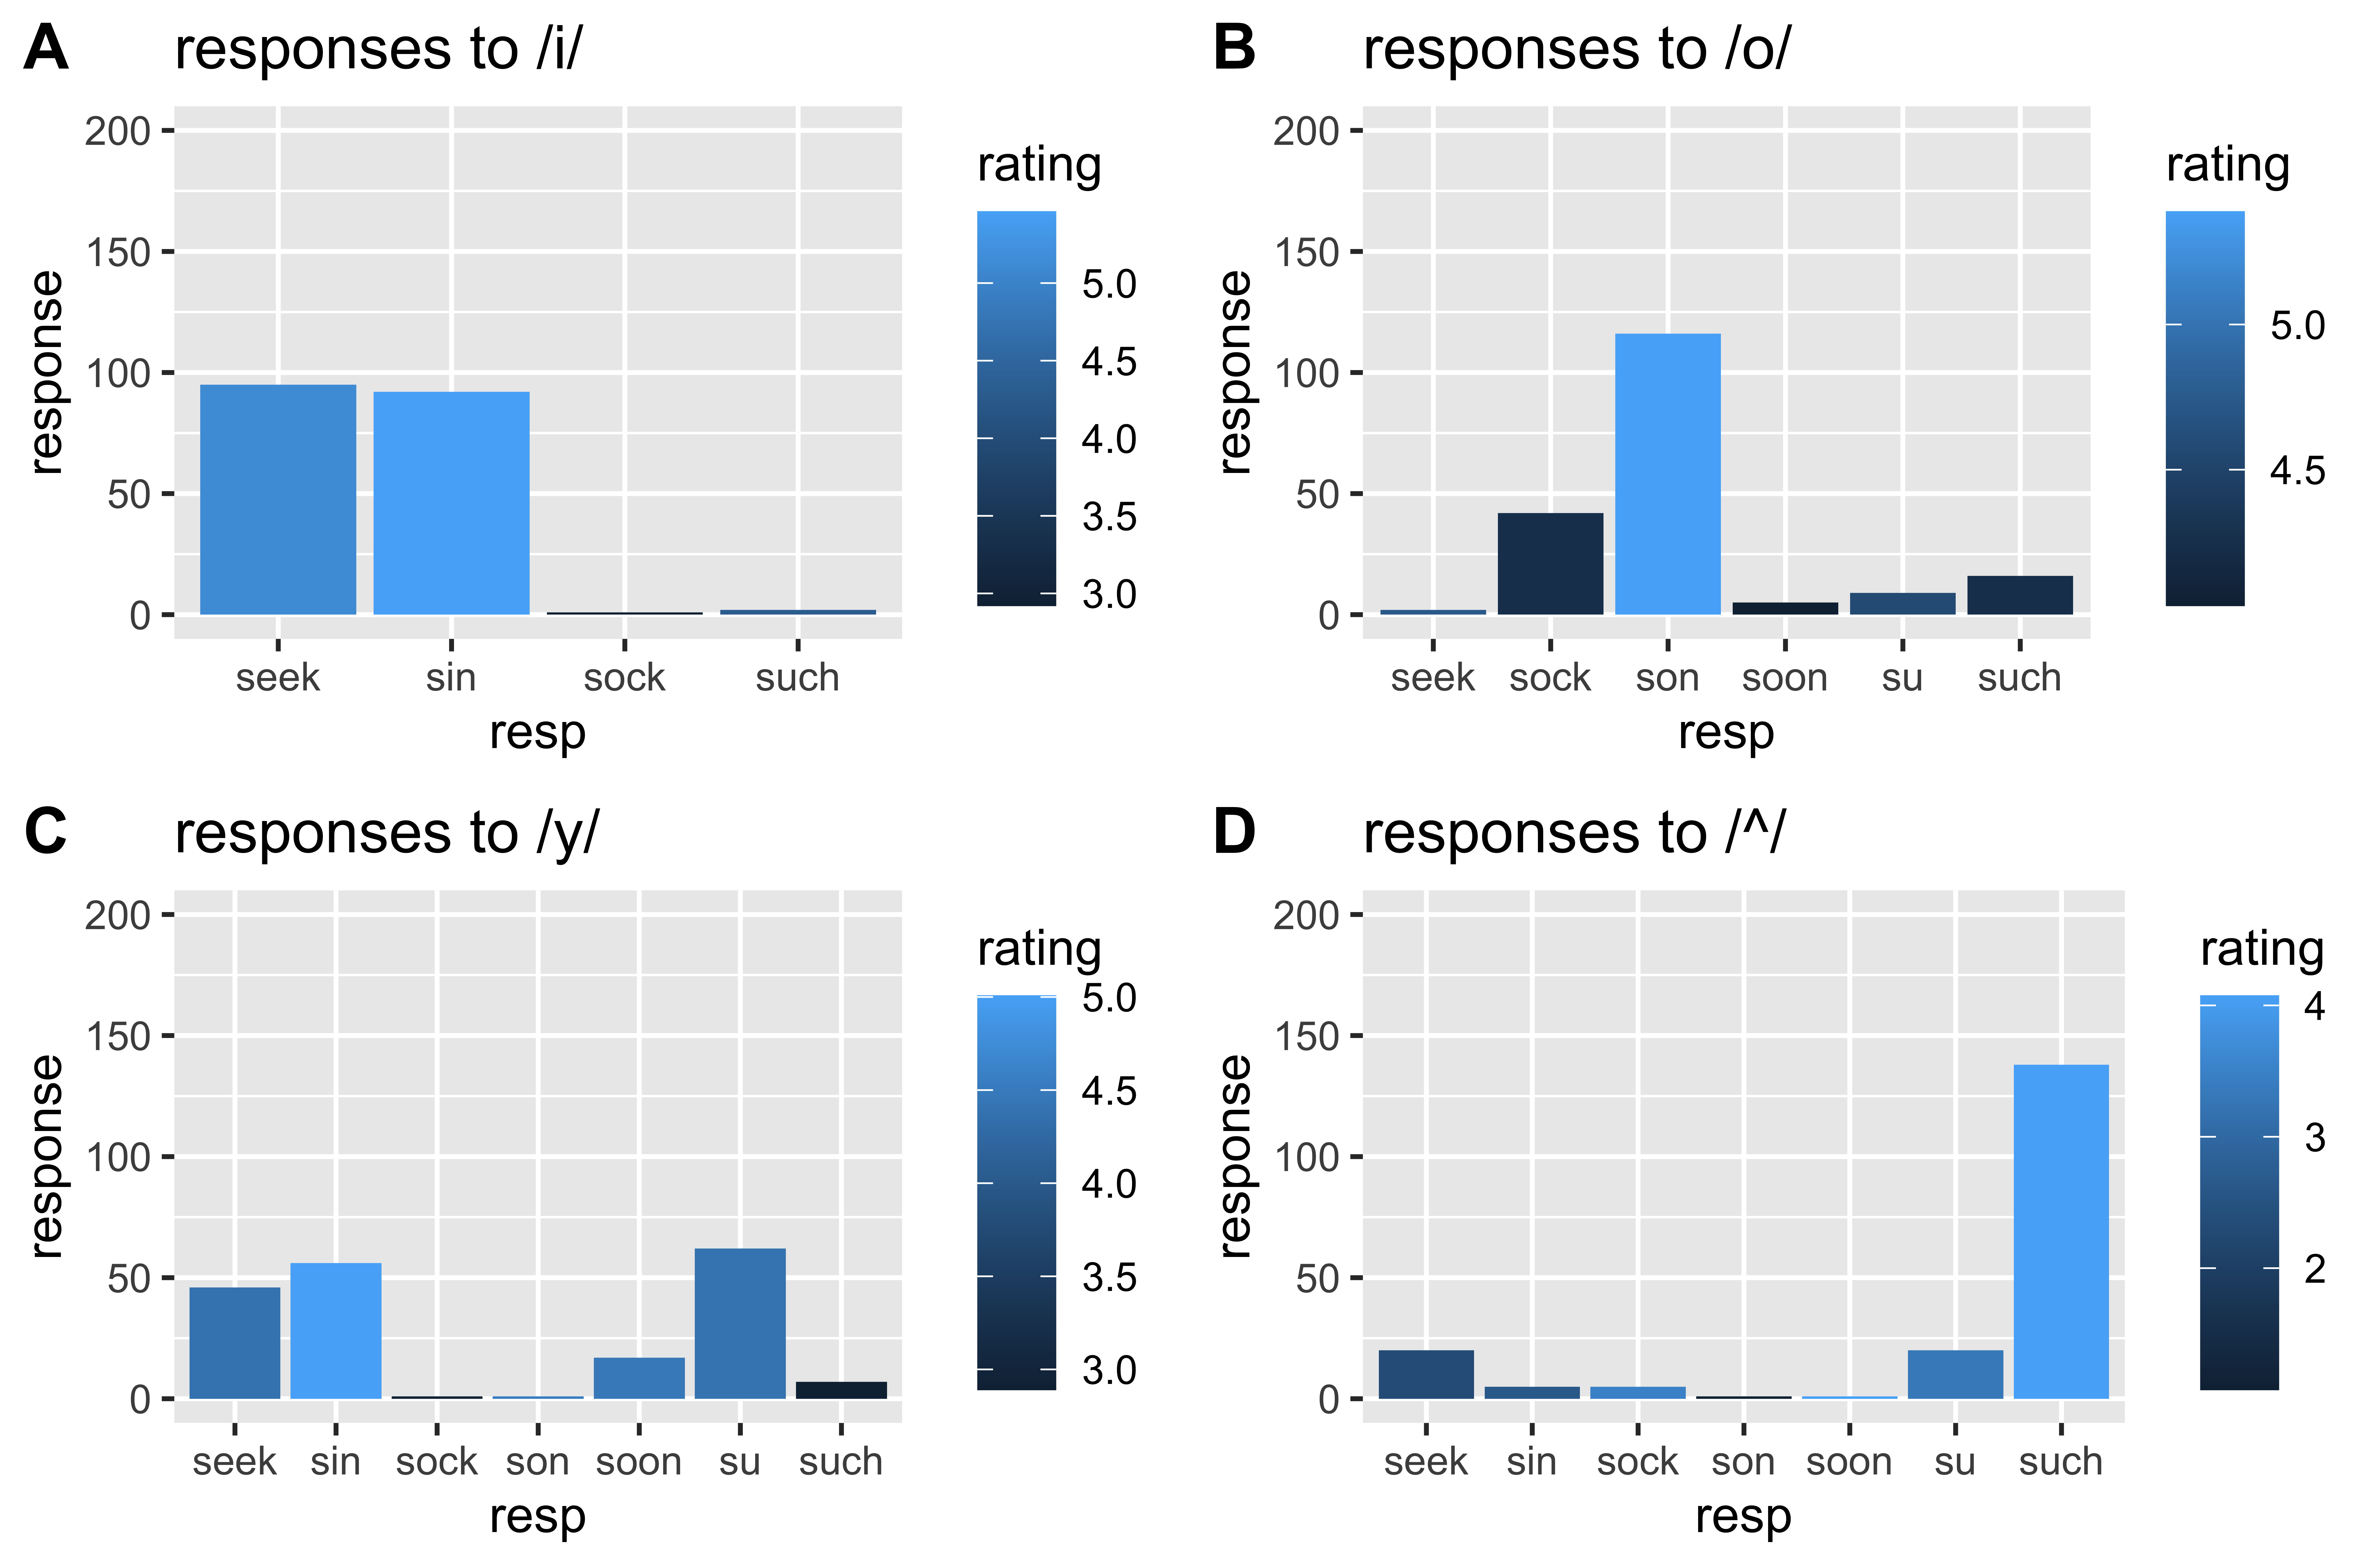
\includegraphics[width=0.9\linewidth,height=0.8\textheight]{/Users/kyleparrish/Documents/GitHub/dissertation_parrish/docs/abstracts/new_sounds/figs/pct_results}

\textbf{Figure 2}

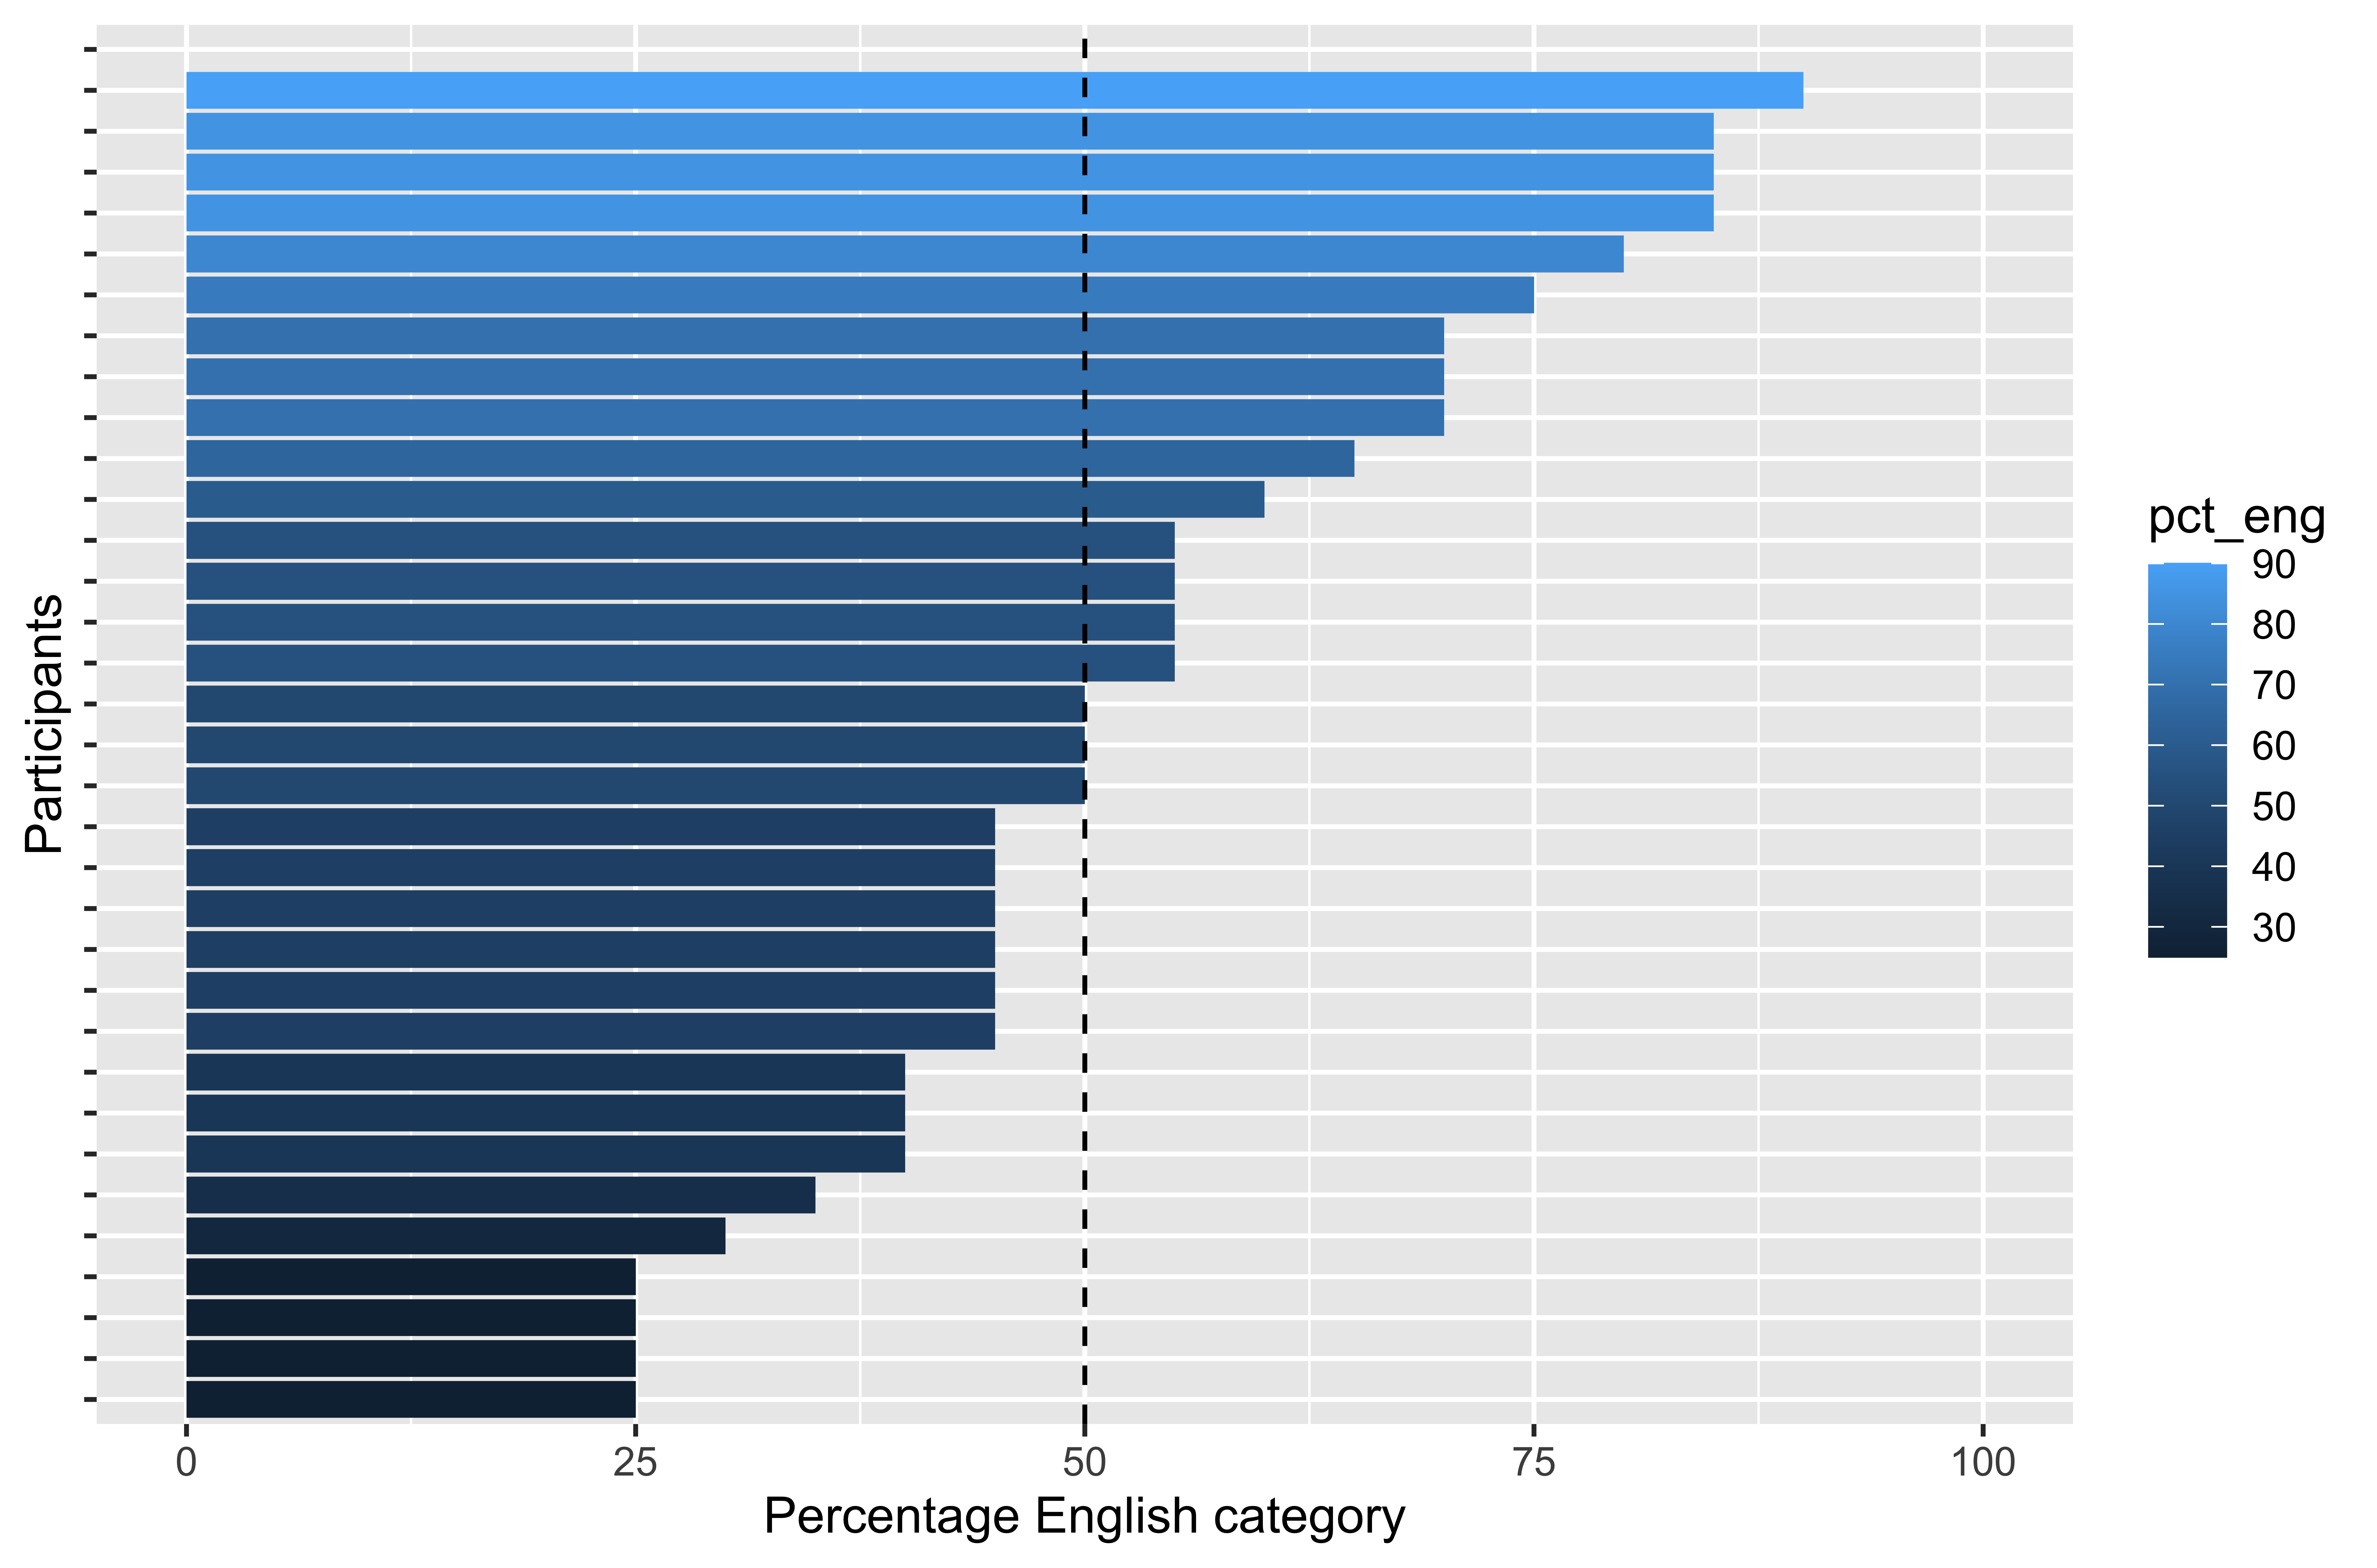
\includegraphics[width=0.9\linewidth,height=0.8\textheight]{/Users/kyleparrish/Documents/GitHub/dissertation_parrish/docs/abstracts/new_sounds/figs/eng_percent}

\hypertarget{references}{%
\subsection{References}\label{references}}

\begingroup
\setlength{\parindent}{-0.5in}
\setlength{\leftskip}{0.5in}
\phantom{.}

\textcolor{white}{\\} \vspace{-0.5in}

Bardel, C., \& Falk, Y. (2007). The role of the second language in third
language acquisition: The case of Germanic syntax. Second Language
Research, 23(4), 459--484.
\url{https://doi.org/10.1177/0267658307080557}

Best, C. T., \& Tyler, M. D. (2007). Nonnative and second-language
speech perception: Commonalities and complementarities. In O.-S. Bohn \&
M. J. Munro (Eds.), Language Learning \& Language Teaching (Vol. 17,
pp.~13--34). John Benjamins Publishing Company.
\url{https://doi.org/10.1075/lllt.17.07bes}

Rothman, J. (2015). Linguistic and cognitive motivations for the
Typological Primacy Model (TPM) of third language (L3) transfer: Timing
of acquisition and proficiency considered. Bilingualism: Language and
Cognition, 18(2), 179--190.
\url{https://doi.org/10.1017/S136672891300059X}

Slabakova, R. (2017). The scalpel model of third language acquisition.
International Journal of Bilingualism, 21(6), 651--665.
\url{https://doi.org/10.1177/1367006916655413}

Westergaard, M., Mitrofanova, N., Mykhaylyk, R., \& Rodina, Y. (2017).
Crosslinguistic influence in the acquisition of a third language: The
Linguistic Proximity Model. International Journal of Bilingualism,
21(6), 666--682. \url{https://doi.org/10.1177/1367006916648859}

\endgroup

\end{document}
